
\chapter{High-Temperature Testing}

In order to effectively test these eutectic alloys, a test facility capable of housing specimens at 1200--1400\celsius\ in an inert atmosphere, and possessing a cross-head that can exert 5kN of force or higher, would be required in the first instance.  Many high-temperature mechanical testing facilities were explored.

Through preliminary compressive and tensile testing, these eutectic alloys were found to have a DBTT of over 1000\celsius.  Inhomogeneous alloy manufacture and the poor finish from EDM machining achieved on test specimens meant that any tensile testing at 1000\celsius\ or under would fail in the elastic regime due to specimen notch sensitivity and brittleness.  Tensile testing would have to be conducted at temperatures above DBTT to obtain pertinent quantitative mechanical data.

The tensile and compressive creep testing facilities in Rolls-Royce have test-chambers that can reach 1200\celsius\ in ambient, not inert, atmosphere.  The compression creep rigs available at the University of Swansea were also unsuitable, as they also do not have the option of having their test chambers housed in an inert atmosphere.  There is an in-house furnace that can reach 2000\celsius\ in vacuum or inert atmosphere.  This did not, and still does not, have a compression rig set-up for it.  There is also an in-house Thermec furnace that can reach 1800\celsius\ in inert atmosphere.  This also did not have sufficient compression capabilities to carry out compression or compression creep testing.

Since there are no facilities available in Europe that can compression test specimens in an inert environment at 1200-1400\celsius, and that the facilities in North America are not readily accessible for this work due to the confidential nature of the project, accessible high-temperature compression facilities without the required capabilities were explored in the first instance.  

In this Chapter, compression tests performed in-house, at the ENGINX beamline of Rutherford Appleton Laboratory (RAL), UK, at the ID15b beamline of the European Synchrotron Radiation Facility (ESRF), and at the Mechanical Engineering Department of Brown University will be described. Tensile test attempts on the in-house Low-Cycle Fatigue (LCF) test-rig, and on the ETMT machines in-house and at the National Physical Laboratory (NPL) will also be detailed.

\section{High-Temperature Compression Testing}\label{chap:highT}
 
Table \ref{tab:compress} lists the capabilities of the various testing facilities used for high-temperature compression testing of the eutectic alloys explored in this project.  The LCF does not have the protective test chamber environment nor the temperature capabilities required for compression testing.  The mirror furnace used to heat the test environment of the Instron machine of EnginX has a maximum temperature capability of 1000\celsius.  
ID15b utilises resistance heating across the sample to heat it up.

\subsection{Testing on the in-house LCF Rig}

The LCF had typically been used for testing of oxidation resistant superalloys at temperatures of up to 750\celsius\ in an open atmosphere (Figure \ref{fig:lcf}).  It has an Instron$^{\textregistered}$ cross-head with a 5kN load cell.  For hot testing, a cylindrical furnace that opens and closes like a clamshell can surround the test area to form a hot test chamber (Figure \ref{fig:lcfhot}). 
As 750\celsius\ is too low for any test of relevance to be conducted in the first instance, the LCF was modified to increase its operating temperature using insulating fibre-glass wool around any gaps around the furnace and test chamber (Figure \ref{fig:lcfcloseup}).  This allowed it to reach a maximum of 980\celsius, but 950\celsius\ was more typical temperature.  A metal tube was inserted into the test chamber enclosed by the cylindrical furnace to trickle in argon gas.  This provided a less oxidising environment to minimise specimen or platen failure due to runaway oxidation.  This set-up is still considered an open environment though. 

Compression tests were performed with platens made of various materials.  All the material was DS, with the exception of V-V$_3$Si , which was PMed.  The process required to get V-V$_3$Si manufactured using the DS process is a protracted process involving manufacturing suitable feedstock for utilising the 4-mirror Xe image furnace at the University of Warwick.  As V-V$_3$Si would not be a viable candidate for use in the hot section of a jet engine due to its propensity for harmful pentoxide formation, it was deemed reasonable to forgo manufacturing V-V$_3$Si via the DS process, and to use PM processed stock instead.  All alloys were multi-grained, as no seed was used as a grain selector during manufacture.  The compression platens were flat discs 5mm tall and 20mm in diameter, with the flat surfaces ground till they were parallel with each other.  Disc superalloy stock of tensile-test-quality was used as platen material due to its ready availability in the lab.  
A cylindrical sample (Figure \ref{fig:testcylinders}) was put between 2 disc platens, and they were then placed on the bottom push-rod.

At 980\celsius, the binary and ternary eutectics deformed the disc superalloy platens (Figure \ref{fig:lcfhotzoom}).  This was the first indicator of the alloy system’s medium temperature properties; despite being merely a qualitative result, it could be said that the DS ternary eutectic alloy is stronger than an advanced powder-process manufactured disc superalloy at 980\celsius.

%
\begin{landscape}
\begin{table}[htdp]
\begin{center}
\begin{tabular}{lccccc}
\hline\hline
Test-Rig 		&  Test Chamber Environment&Temperature Capacity&	Stress-Rig Capacity&	Location	\\
\hline
LCF 		&open-air 	&	to 850\celsius	&  sufficient 	&in-house\\
Instron	&open-air	& 	only to 1000\celsius					&sufficient		&ENGINX, RAL, UK\\
Instron	&inert									&	resistance heating	&sufficient		&ID15b, ESRF, France\\
Bespoke Instron&inert							&up to 2000\celsius						&sufficient		&Brown University,  U.S.A \\
\hline\hline
\end{tabular}
\end{center}
\caption{Description of the compression testing facilities that were used in high-temperature mechanical testing.}
\label{tab:compress}
\end{table}
\end{landscape}


%
\begin{figure}[H]
\begin{center}
\includegraphics[width=8cm]{lcf}
\caption{Photo of the in-house Low-Cycle Furnace with an Instron load-cell at the department.}\label{fig:lcf}
\end{center}
\end{figure}
%
%
\begin{figure}[H]
\begin{center}
\includegraphics[width=6cm]{lcfhot}
\caption{Photograph of the test chamber of the LCF at the end of a compression test.}
\label{fig:lcfhot}
\end{center}
\end{figure}
%
%
\begin{figure}[H]
\begin{center}
\includegraphics[width=8cm]{lcfcloseup}
\caption{Close-up photo of the in-house Low-Cycle Furnace at the department with insulation and extensometer in place.  Glass wool has been stuffed around the openings of the clam-shell furnace to keep the heat in.}\label{fig:lcfcloseup}
\end{center}
\end{figure}
%
%
\begin{figure}[H]
\begin{center}
\includegraphics[width=6cm]{testcylinders}
\caption{Photograph of 3-5mm diameter cylindrical test specimens manufactured by electro-spark machining.}
\label{fig:testcylinders}
\end{center}
\end{figure}
%
%
\begin{figure}[H]
\begin{center}
\includegraphics[width=6cm]{lcfhotzoom}
\includegraphics[width=6cm]{lcfhotzoomii}
\caption{Photographs of cracked disc superalloy platens in the LCF test chamber at the end of a compression test.}
\label{fig:lcfhotzoom}
\end{center}
\end{figure}
%

Tungsten carbide platens were then used.  Tungsten carbide is known for its high-temperature strength.  It forms an oxygen permeable oxide, which leads to runaway oxidation.  This would contribute substantially to inaccuracy in sample strain determination.  In theory, if the platens were exposed to a less oxidising atmosphere with the presence of a steady flow of inert argon gas during the experiment, if the test chamber was padded and stuffed with insulating glass-fibre wool to limit the air circulation within the chamber, and if the duration of oxidation time were to be limited by minimising the amount of time required for temperature ramp-up and cool-down, the platens may not oxidise substantially.  

The test started with the sample showing elastic deformation to 120MPa, upon which a crack was heard, followed by a sudden reduction in load.  This was equated to either the sample cracking, or a component in the rig cracking.  When the rig was cooled and the set-up was examined, it was found that runaway oxidation did occur in the platens.  The voluminous tungsten oxide that formed had cracked, and this crack propagated into the tungsten carbide platen (Figure \ref{fig:wcplaten}), and showed up as load reduction in the test.  The tungsten oxide is covered with a thin layer of vanadium pentoxide which had volatilised from the test specimen and condensed onto the platen (Figure \ref{fig:wcplaten}).  Tungsten carbide platens are thus unsuitable for high-temperature testing in semi-inert atmospheres.  The test specimen looked undeformed and had formed a thin oxide layer (Figure \ref{fig:25V_lcf_950}).  

%
\begin{figure}[H]
\begin{center}
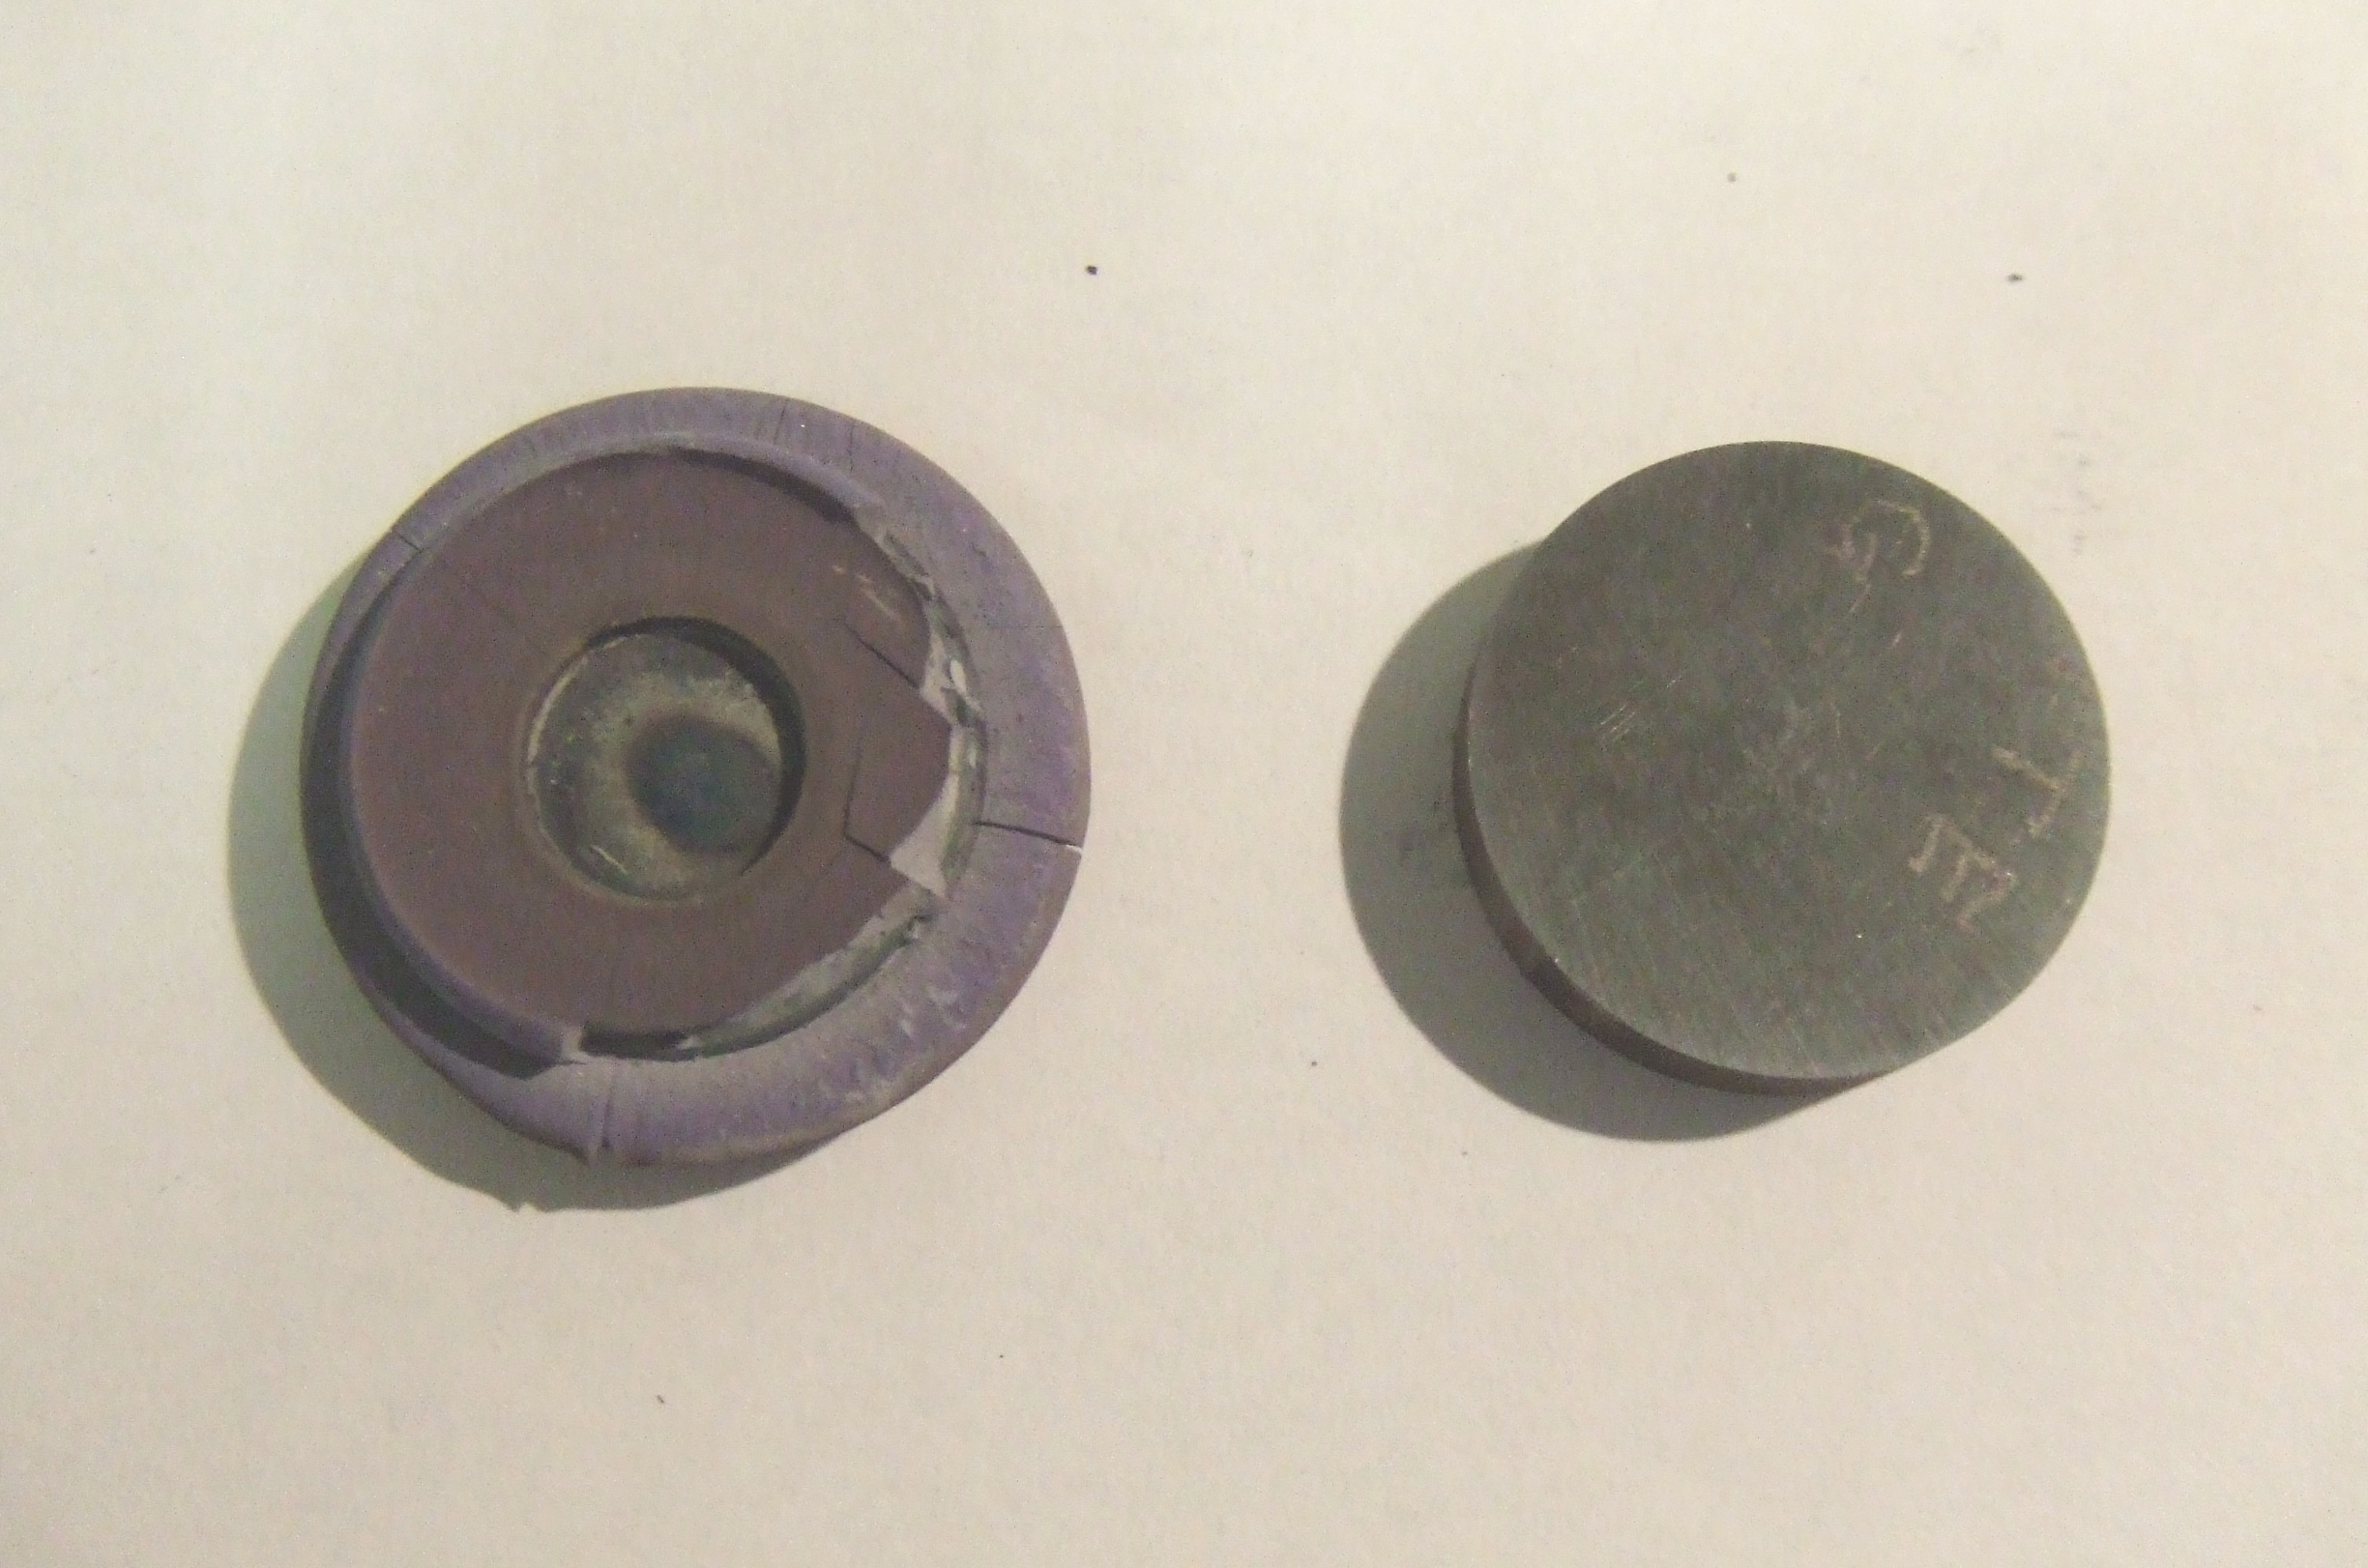
\includegraphics[width=8cm]{wcplaten}
\caption{A photograph of tungsten carbide platens. The left platen underwent one test for a specimen of ($\frac{1}{4}$V,$\frac{3}{4}$Cr)--($\frac{1}{4}$V,$\frac{3}{4}$Cr)$_3$Si at 950\celsius\ (Figure \ref{fig:25V_lcf_950}) and experienced pesting.  The test had to be stopped due to platen cracking.  The right platen is an unblemished tungsten carbide measuring 25mm in diameter and 5mm tall.}
\label{fig:wcplaten}
\end{center}
\end{figure}
%

%
\begin{figure}[H]
\begin{center}
\includegraphics[width=8cm]{25V_lcf}
\caption{A photograph of the specimen of ($\frac{1}{4}$V,$\frac{3}{4}$Cr)--($\frac{1}{4}$V,$\frac{3}{4}$Cr)$_3$Si that underwent an interrupted compression test at 950\celsius. }
\label{fig:25V_lcf_950}
\end{center}
\end{figure}
%

Discs of alumina and zirconia manufactured by slip-casting followed by kiln-firing were custom ordered from Almath Crucibles, a specialist manufacturer in Newmarket, U.K..  Being ceramics, alumina and zirconia exhibit poor fracture-toughness and can crack.  However, they cannot be further oxidised under the set-up conditions.  If no platen cracking is observed after the test, the displacement data of the test would be rendered accurate.  Alumina is stronger, cheaper, but more brittle than zirconia.  Both materials were used to look at their suitability as compression platens.  Both materials were found to work quite well (Figure \ref{fig:lcfsantai}), and the compressive strengths of the binary and ternary alloys could be determined for temperatures between 850 and 980\celsius. 

The two ternaries tested, ($\frac{3}{4}$Cr, $\frac{1}{4}$V)--($\frac{3}{4}$Cr, $\frac{1}{4}$V)$_3$Si and base alloy \ilovewill{山}, were found to be stronger than the vanadium binary at 980\celsius\ (Figure \ref{fig:vcompression}). The vanadium binary underwent pesting during its short test (Figure \ref{fig:vspec}).

It would have been possible to upgrade the clam-shell heater of the LCF to a more powerful heater to achieve higher temperatures, but since the test environment would still remain open-air, where an inert environment could not be constructed, the upgrade was not pursued.

%
\begin{figure}[H]
\begin{center}
\includegraphics[width=8cm]{lcfsantai}
\caption{Photograph of a compression specimen made from  \ilovewill{山}Ta, post-test, with one of its alumina platens that has turned grey due to being covered with oxide from the specimen.}
\label{fig:lcfsantai}
\end{center}
\end{figure}
%
%
\begin{figure}[H]
\begin{center}
\includegraphics[width=12cm]{vcompression}
\caption{Compression testing of V--V$_3$Si at 980\celsius.}
\label{fig:vcompression}
\end{center}
\end{figure}
%
%
\begin{figure}[H]
\begin{center}
\includegraphics[width=10cm]{v_comp_specimen}
\caption{Specimen of V--V$_3$Si that had undergone compression testing (Figure \ref{fig:vcompression}) in the LCF test-rig.}
\label{fig:vspec}
\end{center}
\end{figure}
%



\subsection{Testing at ENGIN--X}

The option of using a high-temperature stress-rig at a British neutron synchrotron beam-line was explored. EnginX is located at ISIS, which is part of the Rutherford Appleton Laboratory in Didcot, England.  There is an Instron stress-rig that is capable of 50kN of force (Figures \ref{fig:enginxbanks} and \ref{fig:enginxloadcell}).  When neutrons were available, an in-situ experiment to quantify the load partitioning between the solid-solution and intermetallic phases was attempted.  This will be discussed in Chapter 8.

The specifications of the 4-lamp furnace used to heat up the test environment state that it is capable of 1100\celsius\ (Figures \ref{fig:enginxfurnace} and \ref{fig:enginxloadedsample}).  This is more than a 100 degrees higher than the maximum temperature of the LCF rig used in the previous section, but may not be high enough for the test samples to move out of their brittle regime.  If the DBTTs of some of the designed alloys are lower than this temperature, then the solid-solution would be in the ductile state, which would allow for plastic deformation to occur.  The test chamber will be sealed with aluminium plates, and Argon was flushed through at 5\litre /minute (Figures \ref{fig:enginxtc}, \ref{fig:enginxvent} and \ref{fig:tubesinvent}).  When in operation, the stress-rig would have a slight, sinusoidal fluctuation in stress, with a period of 20 minutes.  The cause of this is unknown.

%
\begin{figure}[H]
\begin{center}
\includegraphics[width=14cm]{enginxbanks}
\caption{Photograph of the adjustable sample turn-table, beam slits, together with the north and south bank detectors on the EnginX beamline.}\label{fig:enginxbanks}
\end{center}
\end{figure}
%
\begin{figure}[H]
\begin{center}
\includegraphics[width=14cm]{enginxloadcell}
\caption{Photograph of the Instron 20kN load-cell before it was set-up on the adjustable sample turn-table of the EnginX beamline.}\label{fig:enginxloadcell}
\end{center}
\end{figure}
%
\begin{figure}[H]
\begin{center}
\includegraphics[width=14cm]{enginxfurnace}
\caption{Photograph of the halogen-lamp 4-mirror furnace installed to enclose the test environment of the Instron load-cell.}\label{fig:enginxfurnace}
\end{center}
\end{figure}
%
%
\begin{figure}[H]
\begin{center}
\includegraphics[width=14cm]{enginxloadedsample}
\caption{Photograph of a typical DS cast cylindrical sample loaded in compression between bespoke white alumina platens in the Instron load-cell prior to testing.  There is a thermocouple tied to the cylinder's curved surface by platinum wire.}\label{fig:enginxloadedsample}
\end{center}
\end{figure}
%
%
\begin{figure}[H]
\begin{center}
\includegraphics[width=12cm]{enginxtc}
\caption{Photograph of thermocouples and cooling systems the 4-mirror halogen-lamp furnace.}\label{fig:enginxtc}
\end{center}
\end{figure}
%
Specimens were 8\milli\metre\ in diameter and 18\milli\metre\ tall (Figure \ref{fig:enginxsample}).  Volatile oxides exuded by the test specimens were, in the most part, vented to outside the building because dilution is, more often than not, regarded as the best solution to pollution.  A portion of pentoxide and chromia condensed on the water-cooled surfaces in the test chamber.  In Figure \ref{fig:enginxtestedsample}, a green chromia oxide is seen on the sample despite chromia being volatile at 980\celsius, and some form of mixed oxide has condensed on the copper cooling rings placed around the compression grips. Vanadium pentoxide occur as red patches on the previously white alumina platens.
%
\begin{figure}[H]
\begin{center}
\includegraphics[width=9cm]{enginxvent}
\caption{Photograph of the industrial-sized ventilation system installed on the EnginX beamline to extract hazardous oxide emissions out of the building.}\label{fig:enginxvent}
\end{center}
\end{figure}
%
%
\begin{figure}[H]
\begin{center}
\includegraphics[width=14cm]{tubesinvent}
\caption{Photograph of the red tubes used to vent the argon gas required to maintain an inert atmosphere being fed to the ventilation system.}\label{fig:tubesinvent}
\end{center}
\end{figure}
%


%
\begin{figure}[H]
\begin{center}
\includegraphics[width=8cm]{enginxsample}
\caption{Photograph of a \ilovewill{山}Ta compression sample prior to testing.}\label{fig:enginxsample}
\end{center}
\end{figure}
%

%
\begin{figure}[H]
\begin{center}
\includegraphics[width=10cm]{enginxtestedsample}
\caption{Photograph of a \ilovewill{山}Ta compression sample after being subjected to 900\celsius\ for 5 hours.}\label{fig:enginxtestedsample}
\end{center}
\end{figure}
%

\subsubsection{Results}

Compression creep testing was conducted at 910\celsius\ and 1000\celsius\ the Cr--Cr$_3$Si binary and the \ilovewill{山}Ta quaternary.  The binary experienced gradual creep at 910\celsius\ /200MPa over 4 hours (Figure \ref{fig:enginxcr910C200MPa7}) and substantial creep at 1000\celsius\ /200MPa over 3 hours (Figure \ref{fig:enginxcr1000C200MPa7}).  Preliminary testing showed the quaternary alloy to be stronger than the binary, and a higher stress of 308MPa was picked for an experiment at 910\celsius.  The quaternary \ilovewill{山}Ta experienced no creep at 910\celsius\ /308MPa for the first 3 hours (Figure \ref{fig:enginxsanta910C308MPa7}), and may have crept very slightly during the last hour.  At 1000\celsius\ /200MPa, there was substantial creep over 3 hours (Figure \ref{fig:enginxsanta1000C200MPa7}).  A specimen of \ilovewill{山}Ta failed during a creep test through brittle shear.  At 980\celsius, the addition of 10at.\% Ta through the substitution of V does not help depress the DBTT substantially, if at all. 

%
\begin{figure}[H]
\begin{center}
\includegraphics[width=14cm]{enginxcr910C200MPa}
\vspace{-2mm}
\caption{Plot of cross-head displacement vs time for Cr--Cr$_3$Si at 910\celsius/ 200MPa.}
\label{fig:enginxcr910C200MPa7}
\end{center}
\end{figure}  
%
%
\begin{figure}[H]
\begin{center}
\includegraphics[width=14.4cm]{enginxcr1000C200MPa}
\vspace{-2mm}
\caption{Plot of cross-head displacement vs time for Cr--Cr$_3$Si at 1000\celsius/ 200MPa.}
\label{fig:enginxcr1000C200MPa7}
\end{center}
\end{figure}  
%

%
\begin{figure}[H]
\begin{center}
\includegraphics[width=14.2cm]{enginxsanta910C308MPa}
\vspace{-2mm}
\caption{Plot of cross-head displacement vs time for \ilovewill{山}Ta at 910\celsius/308MPa.}
\label{fig:enginxsanta910C308MPa7}
\end{center}
\end{figure}  
%

%
\begin{figure}[H]
\begin{center}
\includegraphics[width=14cm]{enginxsanta1000C200MPa}
\vspace{-2mm}
\caption{Plot of cross-head displacement vs time for \ilovewill{山}Ta at 1000\celsius\ /200MPa.}
\label{fig:enginxsanta1000C200MPa7}
\end{center}
\end{figure}  
%



%\subsection{Testing on the ETMT Machine at the ID15b Beamline at ESRF}

%A series of compression tests at 900\celsius, 1100\celsius, 1200\celsius\ and 1300\celsius\ were attempted on the electro-thermo-mechanical testing (ETMT) rig available at the European Synchrotron Facility.


%\subsubsection{Experimental Set-Up} 

%Cylindrical DS samples were used.  They were quite small, had aspect ratios of 1.8, and diameters between 2.0-3.6\milli\metre.  The aspect ratio had to be between 1.8 and 2.2 in order to prevent sample buckling.

%A thermal camera allowed real-time viewing of the sample during testing.  When there was imperfect contact due to the specimen flat surfaces not being perfectly flush with the flat surfaces of the grips, localised hot zones developed.  Hot zone instability was directly proportional to higher specimen temperature. 

%The thermocouples that had been welded onto the specimens had a tendency to de-bond from the sample surface during testing twice out of every three tests.  Initially, the amplitude of current shunted through the specimen was directly coupled to the temperature read by the thermocouple.  During thermocouple de-bonding, the thermocouple would display a spurious temperature between -50 to 40\celsius.  The ETMT, interpreting this as an apparent precipitous temperature drop, would increase current amplitude to increase sample temperature to the set value.  Sample melt would inevitably follow, resulting in test termination. 

%A very accurate pyrometer was mounted above the sample and provided real-time temperature readings.  Its accuracy stems from being capable of measuring a spectrum of wavelengths emitted by the object being measured.  Pyrometer readings were seen to match thermocouple readings within 1-2\celsius\ when the thermocouple weld had integrity.  If the weld between thermocouple and specimen was poor, the thermocouple would give readings that had an inaccuracy of 50-500\celsius. Manual temperature calibration based on pyrometer readings was found to be the most practical way to maintain the constant temperature required during tests.

%A low initial test temperature of 900\celsius\ was chosen to avoid exacerbation of existing issues that could cause test failure.  A steady temperature ramp was chosen to reduce the probability of thermocouple de-bonding.  Tool steel platens were used initially.  It was said that the platens would not experience temperatures over 1000\celsius, and would thus retain sufficient strength to resist any plastic deformation. For this reason, it was said that platens made of disc superalloy were unnecessary, especially since they were more expensive.  In reality, the tool steel platens were found to undergo plastic deformation and became dimpled at areas in contact with the sample due to the high temperatures and stresses experienced, despite being in good contact with the water-cooled cross-head. Later, molybdenum grips were located and used.  These did not deform at any test conditions used.
%\ilovewill{山}Ta appeared strongest, followed by \ilovewill{山}W, \ilovewill{山}TaAl, \ilovewill{山}. V appeared the weakest.
~~~~~~~~~~~~~
%Figure figx900: Stress vs cross-head displacement at 900\celsius\ for the binary, ternary, quaternary and quinary alloys. howard


%Figure figx1100: Stress vs cross-head displacement at 1100\celsius\ for the ternary, quaternary and quinary alloys.
~~~~~~~~~~~~~

%At temperatures of 1200\celsius\ and above, numerous attempts to stabilise sample temperature proved unsuccessful.  The hot zone was seen to vacillate from one end to the other with no apparent periodicity.  This was observed on the screen display of an optical camera that had an adjustable aperture to allow temperature gradients to show up even at red-hot temperatures..
%Stress vs cross-head displacement at 1200\celsius\ for the ternary, quaternary and quinary alloys?
%**Description of mechanical properties**\
%Table of high temperature properties as seen in ETMT testing.
  
%More drastic measures had to be taken.  Permission was granted to visit Professor K.S. Kumar at Brown University and use his high-temperature mechanical testing facilities.


\subsection{Testing Using a High-Temperature Stress-Rig at Brown University}

Permission was granted to conduct high-temperature structural tests on the ultra-high-temperature stress-rig designed by K. S. Kumar of the Engineering Department at Brown University, USA.  An Instron stress-rig with changeable load-cells of 1kN, 5kN and 50kN was custom-fit with a vacuum box furnace that can reach temperatures of 1800\celsius\ (Figures \ref{fig:brownlab}, \ref{fig:brownfurnace} and \ref{fig:browncontrol}).  This allows the user to have control of the test environment.  It can be a vacuum, an inert atmosphere, or a reducing atmosphere. Compressive, tensile, creep and fatigue tests have been reliably conducted using this stress-rig set-up ~\cite{jain10}.  A thermocouple could be placed on the silicon nitride platens that are in contact with the compression sample, or on the sample itself during tests in tension.

Only compression tests were performed.  They are simpler, and the aim was to obtain a matrix of data to compare the structural properties of the alloys that have been designed in this project.  Perhaps the creep exponents some of the alloys could be calculated if sufficient data was collected at different temperatures.  Tensile testing is trickier, and the amount of time required for set-up would be substantially longer than for compression testing. Furthermore, the production of poor specimens was an issue with available DS facilities.  Tensile tests may end up measuring the effect of sample imperfections, which is not the current main focus.  In the short span of time available on the test rig, it seemed sensible to perform simple, short compression tests.  Test temperatures were mostly at 1200\celsius, with a couple of tests at 1300\celsius.  Specimens had a 1.8 height to diameter ratio, and had diameters of 3-5mm.  Some were manufactured by EDM at Electroform, U.K.  And some at the EDM facility at Brown University.  Due to the nature of EDM manufacture, all cylindrical samples had burrs on the flat surfaces, and especially on the curved surface.  The burrs on the flat surfaces had to be removed in order to ensure that both flat surfaces were parallel to each other for the compression test. Each specimen requiring a de-burr was placed in a bespoke jig, held in place using a nylon screw.  These jigs were made at the workshop at the Department of Materials, University of Cambridge.  Their burrs were then slowly ground down lightly using 800-grit polishing paper with water as lubrication.  This method consistently allowed for a flat surface that was square to the curved surface to be achieved during polishing.  Specimens were not skewed during polishing, despite their very small sizes.

%
\begin{figure}[H]
\begin{center}
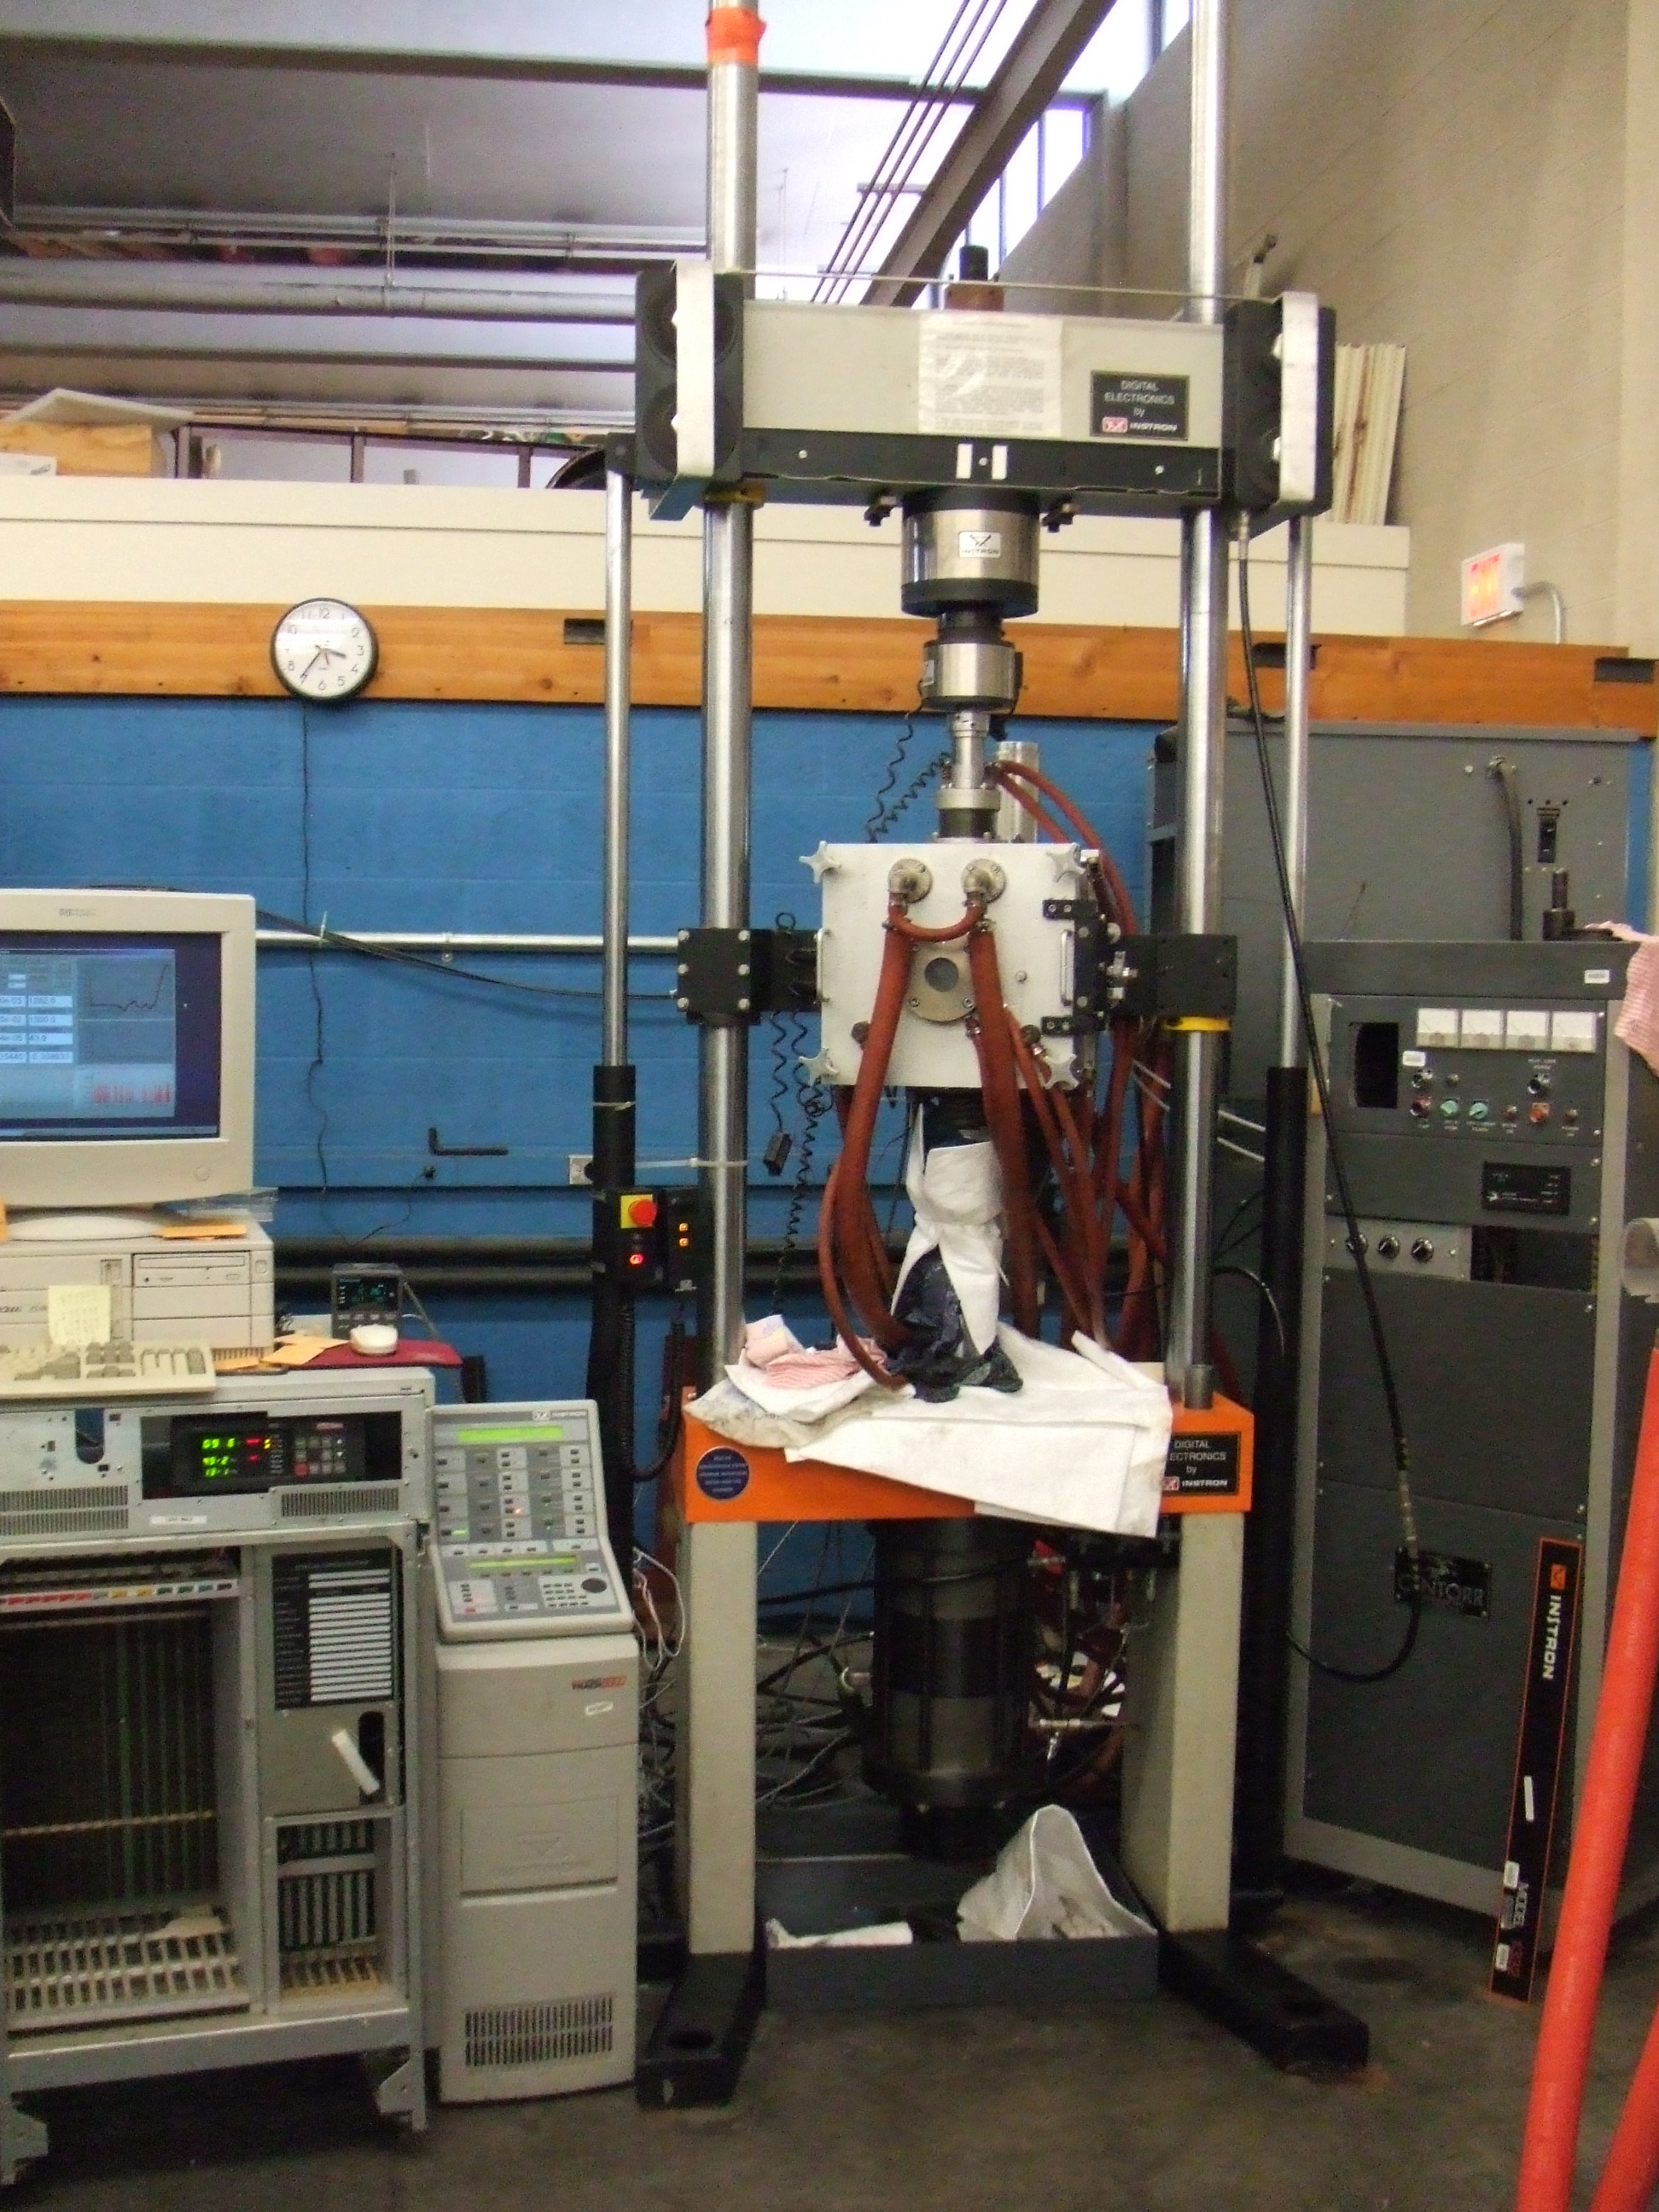
\includegraphics[width=8cm]{brownlab}
\caption{Photograph of the bespoke ultra-high-temperature lab at Brown University with a 5kN load cell attachment.}\label{fig:brownlab}
\end{center}
\end{figure}  
%
%
\begin{figure}[H]
\begin{center}
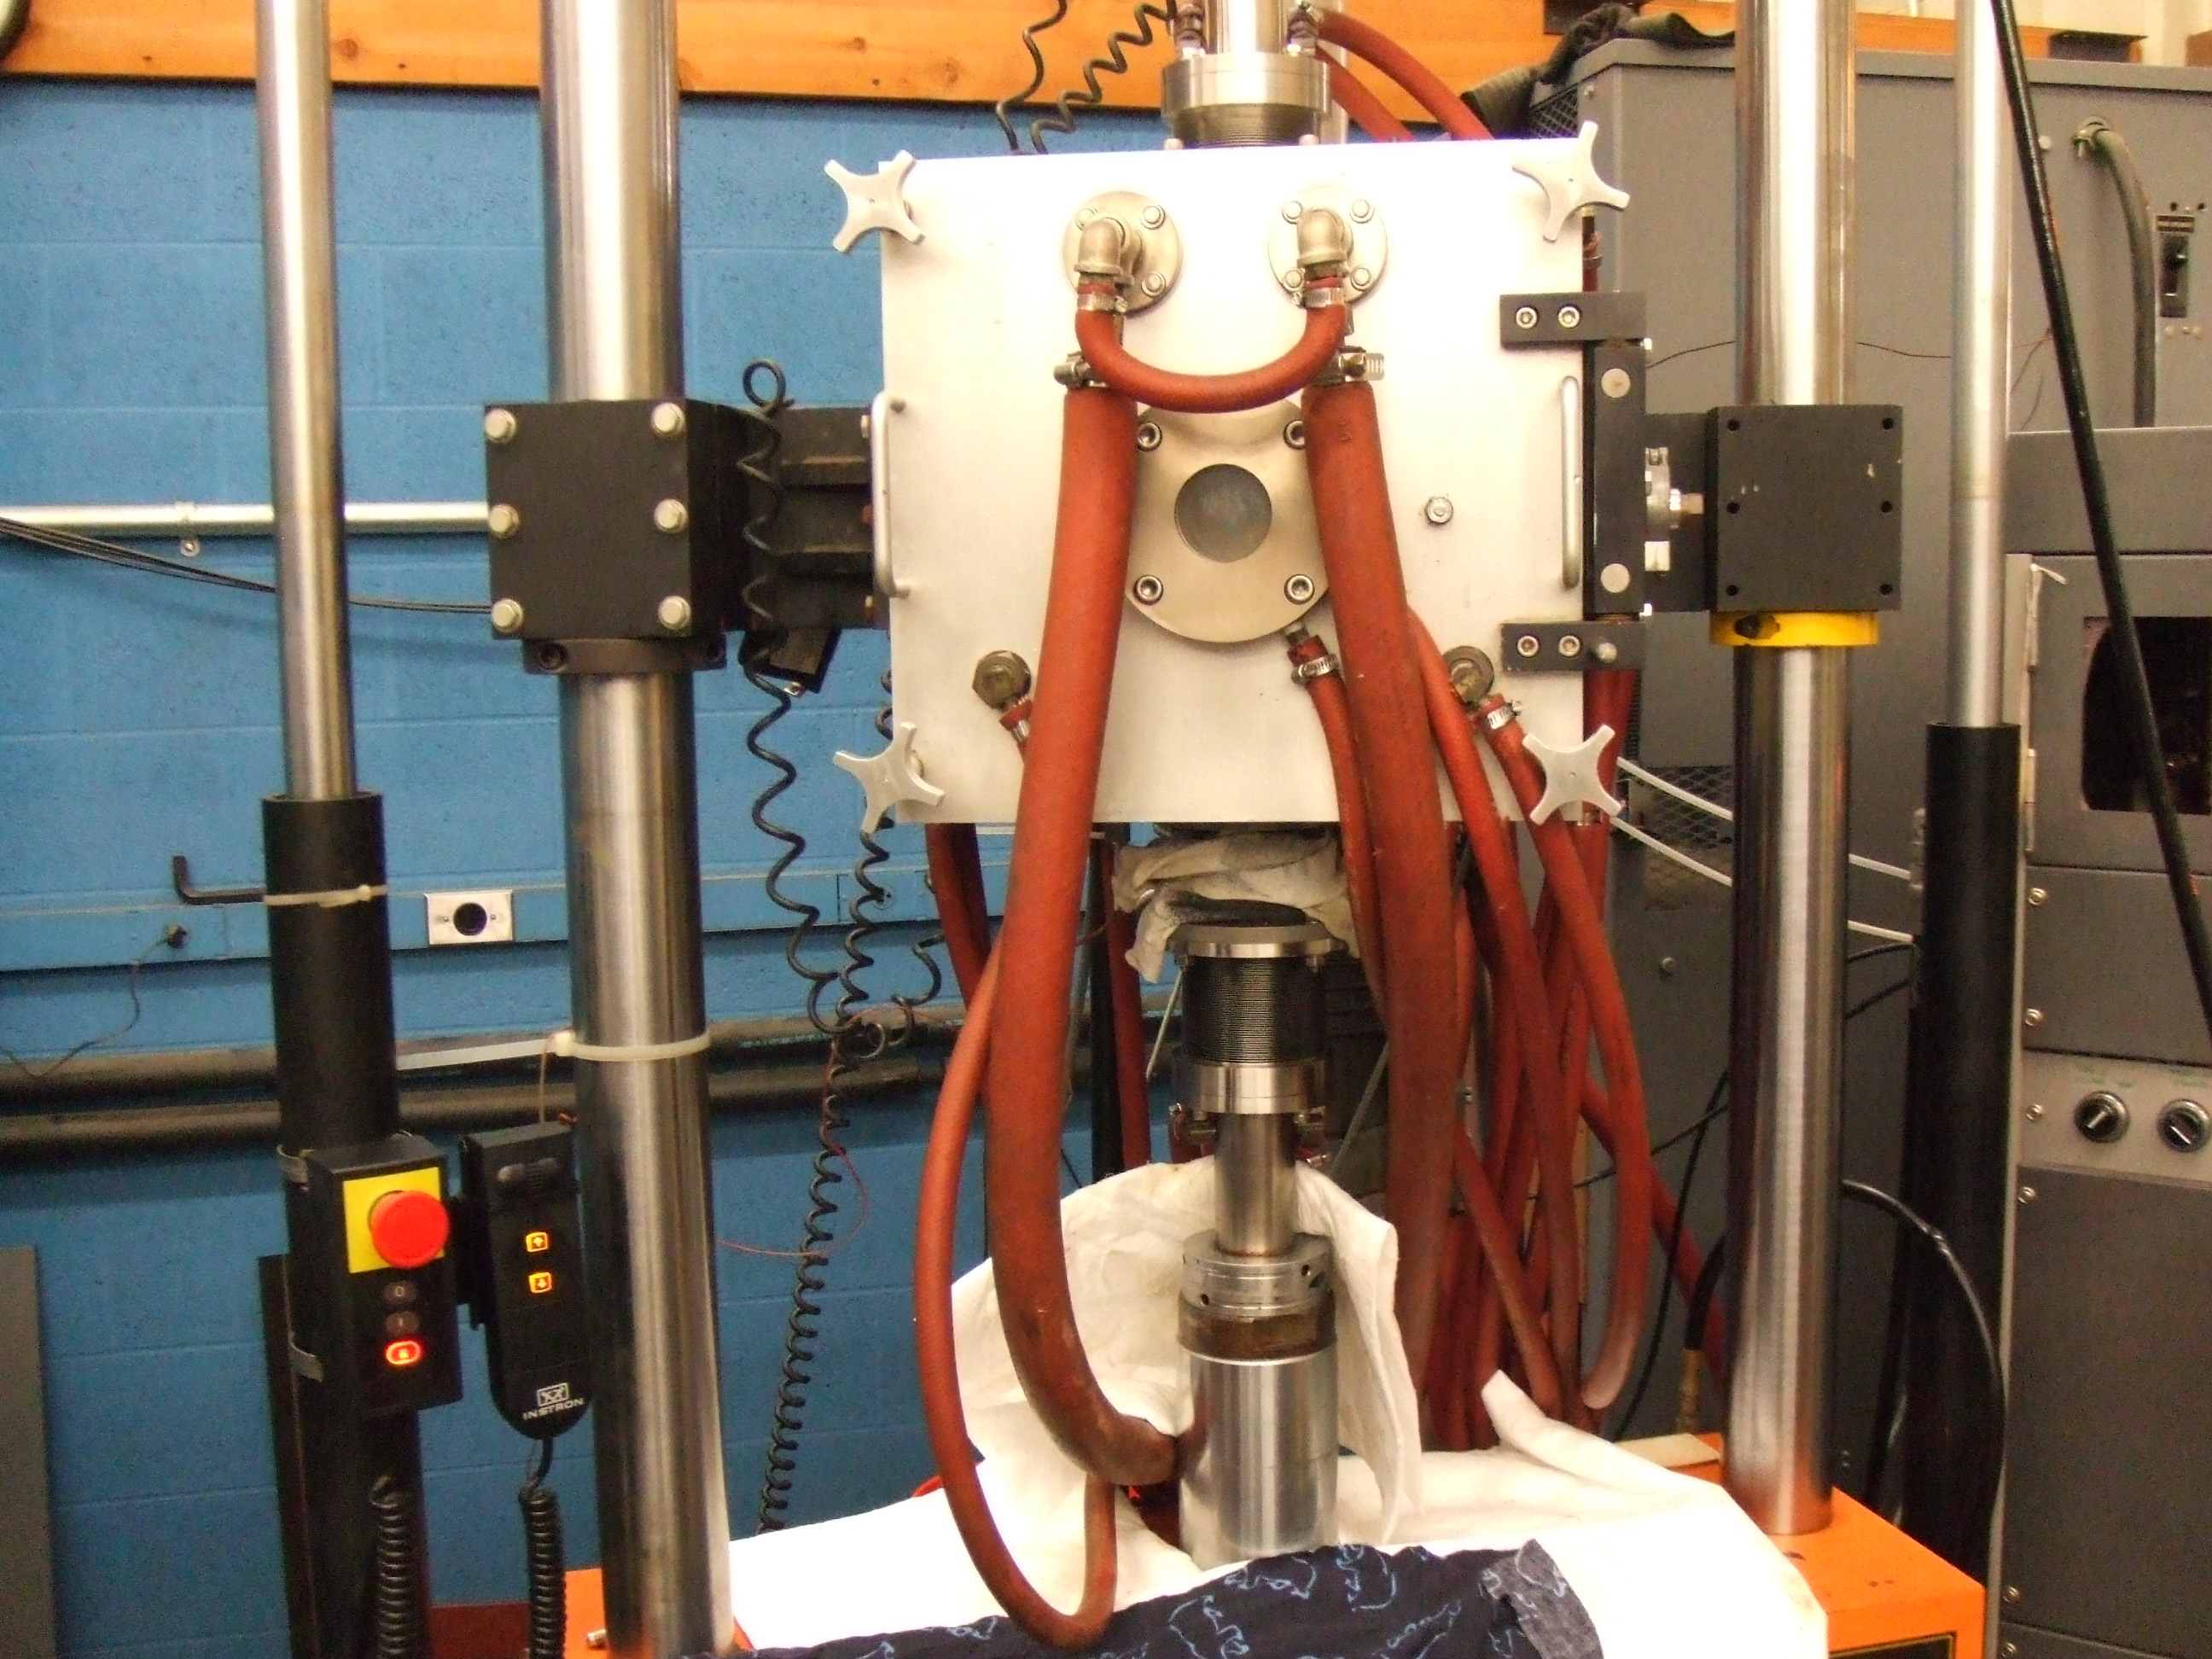
\includegraphics[width=10cm]{brownfurnace}
\caption{Photograph of the bespoke ultra-high-temperature furnace at Brown University with a 5kN load cell attachment.}\label{fig:brownfurnace}
\end{center}
\end{figure}  
%
%
\begin{figure}[H]
\begin{center}
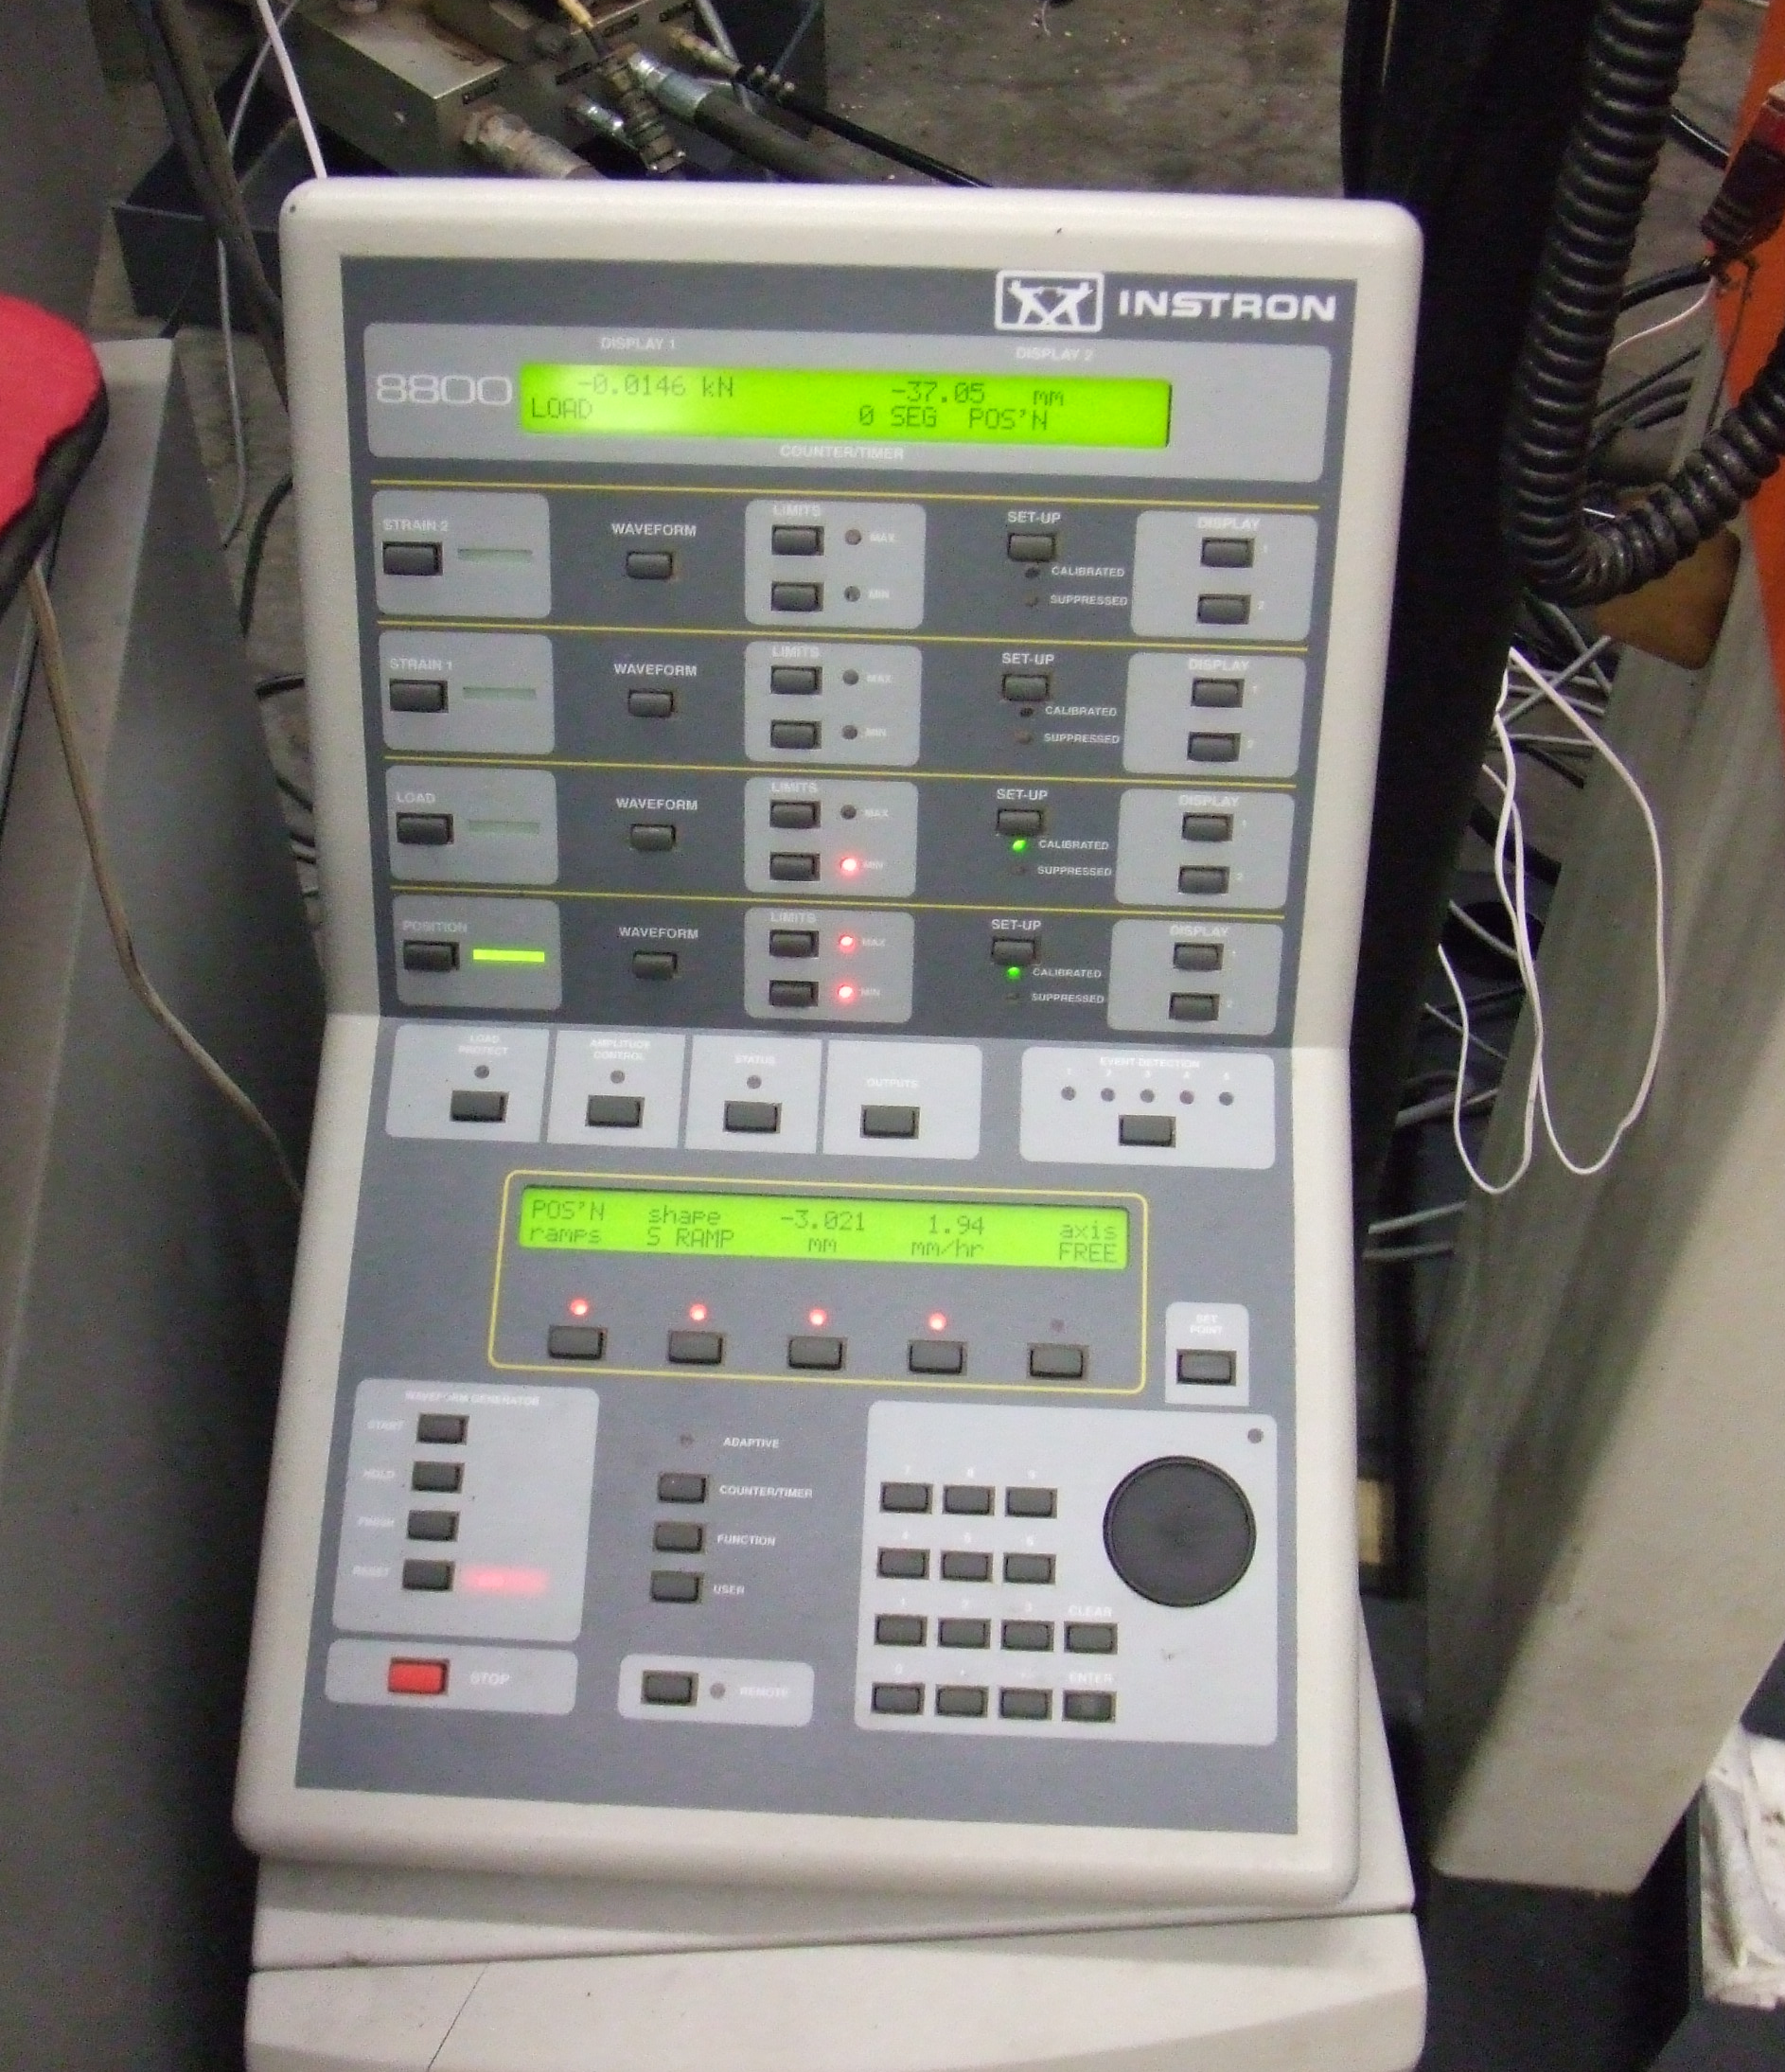
\includegraphics[width=8cm]{browncontrol}
\caption{Photograph of the Instrom control panel of the load cell bespoke ultra-high-temperature stress-rig at Brown University with a 5kN load cell attachment.}\label{fig:browncontrol}
\end{center}
\end{figure}  
%



During the test, the de-burred specimens were placed between SiN platens in the furnace under vacuum.  They were subject to strain rates of 10$^{-4}$/s and 10$^{-5}$/s using an Instron stress-rig fitted with a 5kN load-cell. 

The total length of the cross-head was about 2 metres.  The cross-head rods have diameters of about 10cm, which is very much greater than the test specimens.  The total displacement required to induce 2-5\% plastic deformation in the test specimens would be less than 1 mm.  The cross-head would encounter very much lower stresses, and remain in the elastic regime during loading.  If this reasonable assumption is true, then any plastic deformation would occur only in the sample during the test.  The cross-head displacement was calibrated to show the total displacement generated by the SiN platens and the sample.  The SiN platens are square tiles 20\milli\metre\ by 20\milli\metre\ by 5\milli\metre\ high, and are much harder than the alloys being tested. 

Slight chipping and dimpling were observed in the platens after they were subjected to eight compression tests.  If the flat surfaces of the test cylinders are not perfectly square with the platens, during the onset of loading, one platen would be in contact with one edge of the test cylinder.  This would be akin to using an edge indenter to indent the platen.  A small notch in the brittle ceramic platen could be created, and cracks can propagate from this nucleation site.  The silicon nitride platens are also brittle in nature, and pre-existing cracks can easily propagate when large stresses are applied.

Several samples looked more shiny and cleaner after testing. Under a vacuum atmosphere, volatilisation of vanadium pentoxide was curtailed.  It has the tendency to condense on the inside of the water-cooled furnace door and the water-cooled cross-head, which allowed the extent of pentoxide volatilisation to be monitored.  It was found that runaway oxidation did not ensue under a vacuum atmosphere.  Without runaway oxidation, sample cross-sectional area is not reduced and oxidation’s contribution to test inaccuracy is minimal.

All samples had several grains in each of them.  All binary and ternary samples were DS processed using the in-house RF furnace, except for V--$_3$Si.  Only one bar of V--V$_3$Si had any directionality to it. This was manufactured by crystal-pulling using the 4-mirror furnace at the University of Warwick, but this was used to manufacture tensile test specimens.  No more crystal-pulled V--V$_3$Si stock was left for compression testing.  Specimens were made out of V--V$_3$Si PM manufactured ingots instead.  These specimens are have a finer eutectic structure due to the faster solidification rates encountered during manufacture.  As this eutectic structure is rather globular and less lamellar as the Cr-rich eutectics, the finer microstructure is probably stronger at high temperature. 

The vanadium binary is half as strong as the chromium binary in 10$^{-4}$/s compression tests at 1200\celsius\ (Figure \ref{fig:graph1_1}).  It is suspected that the unrefined lamellae of V$_3$Si did not manage to become the load-bearing phase, and deformation was due to solid-solution flow. If the specimen had been manufactured from a crystal-pulled ingot, its microstructure would probably perform poorly, behaving akin to m\&m's in peanut butter at high temperature.  \ilovewill{山} is much stronger than the binary alloys at 1200\celsius.  The two other intermediate ternary compositions  are not as strong as \ilovewill{山} when tested under the same conditions (Figures \ref{fig:1200e-4qq} and \ref{fig:binaryternary1200e-4}).  In fact, ($\frac{3}{4}$Cr, $\frac{1}{4}$V)--($\frac{3}{4}$Cr, $\frac{1}{4}$V)$_3$Si had same the max stress as Cr--Cr$_3$Si. solid-solution hardening due to vanadium's contribution should have increased its solid-solution high-temperature strength, and thus its overall strength.  It is suspected that all the eutectic alloys of this system have their creep-rates governed by solid-solution flow, and that no plastic deformation occurs in the intermetallic phase.



\subsubsection{Results and Post-Mortem Analysis}

Post-mortem analysis is required to determine why this is so, as solid-solution strengthening cannot account for the increase in strength.  At 1200\celsius\ 10$^{-4}$/s, the maximum compressive stress of 524\mega\pascal\ for \ilovewill{山} is higher than 383\mega\pascal\ for \ilovewill{山}Ta (Figures \ref{fig:sansanTa1200e-4} and \ref{fig:1200e-4}).  The test result for \ilovewill{山}TaAl was discarded as it was made invalid by a machine fault that occurred during testing.  In 10$^{-4}$/s tests at 1300\celsius, \ilovewill{山} and \ilovewill{山}Ta have very similar compression curves, with maxima at 191 and 184\mega\pascal.  As seen in Figure \ref{fig:sanTaii}, \ilovewill{山}Ta solidifies with dendrites of both phases.  If there were only intermetallic dendrites, the alloy would be stronger than if the alloy were to be purely eutectic.  However, solid-solution dendrites would be sites susceptible to localised plastic deformation and be the weak spots in the alloy.  The lamellar microstructure and silicide dendrites thus cannot pick load up effectively.

\ilovewill{山}Ta performs poorly in 10$^{-4}$/s tests at 1200\celsius.
\ilovewill{山}TaAl is the strongest alloy at 1300\celsius, with a maximum stress of 300\mega\pascal\ (Figure \ref{fig:sansanTasanTaAl1300e-4}).  The homogeneous microstructure that could form due to the reduction of melt viscosity from Al's contribution must have allowed the specimen to withstand a higher load.

Solid-solution hardening plays a role in the ternary alloys.  In the quaternary alloy \ilovewill{山}Ta, it should have better high-temperature creep properties because Ta is a potent strengthener of the ductile phase at high temperature.  In a specimen of \ilovewill{山}Ta that did not contain the nominal Ta content due to segregation during manufacture, its resistance to compression at high temperature was similar to that of \ilovewill{山}.

Solid-solution plastic deformation is driven by dislocation flow.  In ordered material such as silicides, it is not necessary to have dislocation-driven plasticity.  At 1200\celsius, the silicide components of these alloys should still be under their DBTTs.  However, it seems that the silicide phase in these alloys are not participating in the uptake of load when compressed.  

These alloys are substantially structurally weaker than HIP manufactured Mo--Si--B alloys designed by Kumar ~\cite{jain10, alur04}.  A two-phase Mo solid-solution + T$_2$ alloy and a three-phase Mo solid-solution + T$_2$ + Mo$_3$Si alloy were compared to a commercially available powder-metallurgy-processed alloy, TZM.  These alloys were isothermally forged.

%~*~*~*~~*~*
%Have to find tensile data for single phase cr and v. 
%flow stress (function of strain rate),  or yield strength. 
%Steve Roberts on cr  alloys and bcc alloys (oxford).
%~*~*~*~*~*~*

%If vanadium is more ductile and not as strong at high temperature than Cr, this could explain why the V--V$_3$Si specimens have such low high-temperature strength.  
%Silicide high-temperature strength.  
%In composites, the ductile phase takes deformation, and limited by the presence of silicides.

If vanadium is softer, we would be able to say with confidence that the material is deforming by solid-solution flow, since the V--V$_3$Si binary is weaker at 1200\celsius\ than the Cr--Cr$_3$Si binary.  Since the range of interlamellar spacings in the ternary and quaternary alloys fall between those of the binaries, it would follow that the quaternary and ternary alloys could be stronger than both binaries due to solid-solution hardening.  If this is the case, this would mean that the silicide phase is probably not taking up load effectively.  Hence, although V$_3$Si has been reported to have higher hot hardness than Cr$_3$Si, and hot hardness has been shown to be directly correlated to high-temperature strength, V$_3$Si's better high-temperature strength is quite irrelevant in these alloys, as the X$_3$Si does not effectively take up the load when in this coarse lamellar configuration. 

If V is harder, then the explanation is not straight forward.  \ilovewill{山}Ta is deforming at the solid-solution dendrites. If it only formed silicide dendrites, it would probably be stronger.

%
\begin{figure}[H]
\begin{center}
\includegraphics[width=10cm]{graph1_1}
\caption{Stress-strain curves of binaries and base-alloy \ilovewill{山} in 10$^{-4}$ compression tests at 1200\celsius.}
\label{fig:graph1_1}
\end{center}
\end{figure}
%
%
\begin{figure}[H]
\begin{center}
\includegraphics[width=14cm]{1200e-4qq}
\caption{Stress-strain curves of all binaries and ternaries in 10$^{-4}$/s compression tests at 1200\celsius.}
\label{fig:1200e-4qq}
\end{center}
\end{figure}
%
%
\begin{figure}[H]
\begin{center}
\includegraphics[width=9cm]{binaryternary1200e-4}
\caption{Plot of maximum stress of the binary and ternary alloys in the 10$^{-4}$/s compression tests at 1200\celsius\ seen in Figure \ref{fig:1200e-4qq}.}
\label{fig:binaryternary1200e-4}
\end{center}
\end{figure}
%
%
\begin{figure}[H]
\begin{center}
\includegraphics[width=8cm]{sansanTa1200e-4}
\caption{Stress-strain curves of base alloy \ilovewill{山} and \ilovewill{山}Ta in 10$^{-4}$/s compression tests at 1200\celsius.  It will be shown in the next Section that the test results for \ilovewill{山} are invalid because the specimen composition is very close to that of Cr--Cr$_3$Si; hardly any V and Ta is present.}
\label{fig:sansanTa1200e-4}
\end{center}
\end{figure}
%
%
\begin{figure}[H]
\begin{center}
\includegraphics[width=14cm]{1200e-4}
\caption{Stress-strain curves of \ilovewill{山}, quaternaries and quinaries in 10$^{-4}$/s compression tests at 1200\celsius.}
\label{fig:1200e-4}
\end{center}
\end{figure}
%
%
\begin{figure}[H]
\begin{center}
\includegraphics[width=10cm]{sansanTasanTaAl}
\caption{Stress-strain curves of base alloy \ilovewill{山}, \ilovewill{山}Ta and \ilovewill{山}TaAl in 10$^{-4}$/s compression tests at 1300\celsius.}
\label{fig:sansanTasanTaAl1300e-4}
\end{center}
\end{figure}
%

In Section 2.2.4, coherent rafts of $\gamma$' in $\gamma$ solid-solution were shown to be effective at impeding dislocation motion in superalloys at high temperature.  Superalloys that form coherent rafts are resistant to high-temperature creep.  Incoherent rafts, such as those in LDSX--8, led to premature rupture in high-temperature tensile creep.  Also, superalloys that form rafts perpendicular to, instead of along, the direction of force have superior high-temperature mechanical properties.  

The intermetallic phase grows along the direction of loading.  The microstructure of the eutectic alloys are an order of magnitude coarser than SX superalloys.  This makes it harder for dislocations to enter the intermetallic phase, and less effective load partitioning would result.  The interface between the solid-solution and intermetallic phases in the X--X$_3$Si alloys is incoherent.  Although there is a slight orientation relationship between these two phases, this is not strong enough to result in a sufficiently coherent interface coherent for dislocations to enter the intermetallic phase.  Consequently, the intermetallic phase is unable to effectively participate in load-bearing, and plastic deformation only occurs in the solid-solution phase.  When the alloy is brought to high temperatures of 1200\celsius, the solid-solution is above its DBTT.  This leads to poor alloy mechanical properties being displayed.  Powder-HIP manufactured alloys from other silicide systems possess substantially better properties an order of magnitude or more ~\cite{jain10}.

\ilovewill{山}W, despite having a seemingly inferior coarse dendritic microstructure, performs substantially better than all lamellar alloys tested.  Having an unrefined microstructure does not affect the structural performace at 1200\celsius\ as much as appropriate alloying.  This is probably due to the intermetallic phase being ineffective in taking up the load.

\subsection{Post-Mortem Analysis of Compression Tested Specimens}

The cylinders were very carefully sectioned using electro-discharge machining.  A vice was custom-made to grip the very small samples to prevent losing samples.  The sections that were made were left on the initial cylinder with about 0.2mm of material left uncut.  When machining was complete, the cylinders were carefully lifted out of the water tank.  The machined sections were then pried by hand.  This was done to prevent losing the tiny millimetre-sized sections in the large water tank filled with machining debris.  Such small sections are difficult to contain and locate when completely detached from the original cylinder. Being light and having high surface areas, they are easily caught by the turbulent water stream and carried away from the catchment tray, to the bottom of the water tank.  As only one sample from each alloy was tested at each compression testing condition, valuable post-mortem data would thus be lost.
	
One longitudinal section through the middle, two transverse sections through the middle, and one transverse section through a quarter of the way through were cut.  The EDM wire erodes a 0.3mm thick section of material with each cut, and the cuts were made to compensate for such a loss in order to get a representative cross-section of the middle of the cylinder.

How would \ilovewill{山}Ta deform? It has a very inhomogeneous microstructure that stems from its highly viscous melt, with dendrites of both solid-solution and silicide, together with two distinct populations of eutectic. 

Case one: the solid-solution dendrite undergoes plastic deformation while everything else stays in the elastic regime.  Should be able to see deformation in dendrites while everything else remains equiaxed.

Case two: if one eutectic population is weaker than the other, the weaker population would deform around the stronger population.  The latter would remain undeformed as it would still be in its elastic regime. The assumption of treating each composite eutectic cell as single-phase is useful.  It would be interesting to look at grain-boundary behaviour during loading.

At low temperatures, grains would not rotate at 4\% total strain.  At 1200\celsius, this is a possibility.  In order to show this, one can take a compression cylinder sliced length-wise into half to look for this.  Unfortunately, the \ilovewill{山}Ta specimen that had undergone 10$^{-4}$/s test compression testing at 1200\celsius\ did not contain Ta and had low V content.  It had a composition very close to the binary alloy Cr--Cr$_3$Si, and thus did not have typical microstructure of \ilovewill{山}Ta (Figure \ref{fig:sanTaRFi}).  The mechanisms of how \ilovewill{山}Ta deforms could not be observed in the post-mortem specimen.  

The PM manufactured feedstock used for DS manufacture was found to have melted incompletely, with extensive segregation present.  Despite using EDS to determine the sections of ingot that had compositions close to nominal composition in order to use them for feedstock, this DS manufactured test specimen was substantially off-composition.  This explains why \ilovewill{山}Ta performed worse than expected in 10$^{-4}$/s tests at 1200\celsius.  Its composition was akin to that of \ilovewill{山}; this caused its mechanical properties to be similar to \ilovewill{山} as well.

The untypical composition of  the \ilovewill{山}Ta specimen means that \ilovewill{山}TaAl has comparatively good structural properties due to the solid-solution effect of Ta, as Al is known to have an adverse effect on the high-temperature mechanical properties of solid-solutions.  

%
\begin{figure}[htbp]
\begin{center}
\includegraphics[width=8cm]{CrVTaRFi}
\caption{Area used for individual phase analysis in \ilovewill{山}Ta.  Although this microstructure is coarse enough for individual phase analysis, no Ta is present.}\label{fig:sanTaRFi}
\end{center}
\end{figure}
% 


%
\subsubsection{Post-Mortem Microstructural Analysis of Compression Tested \ilovewill{山}Ta}

A cylindrical specimen of \ilovewill{山}TaAl that had undergone compression testing at 10$^{-5}$/s at 1200\celsius\ was spark-machined into two halves cut transversely (Figure \ref{fig:graph1_1BSE}).  One half cut longitudinally to access microstructure in a longitundinal section.  The other half was cut into half transversely again to see if different deformation mechanisms could be spotted in the centre and away from the centre of the specimen.

No dendrites were spotted in the specimen (Figure \ref{fig:manual_14_iv_trans_zoomout}).  The specimen may have been cut from a DS bar that had no dendrites in it.  The specimen seemed to have undergone microstructural coarsening during testing (Figure \ref{fig:manual14_v}).  There is only one eutectic morphology present, unlike the different eutectic populations present in the PM and DS manufacture samples.  This different microstructure was found to be due to a composition that was atypical of \ilovewill{山}Ta; there were negligible V and Ta contents (Table \ref{tab:postmortemsanTa}).  The specimen is mostly composed of the Cr--Cr$_3$Si eutectic.  The data shows a very narrow composition range.  Feedstock used in the DS manufacture of this ingot must have had correspondingly low Ta and V content.  This occurred despite conducting EDS and WDS analysis on the sectioned PM manufactured ingot to determine the regions to obtain feedstock for DS manufacture.  This eutectic microstructure does not resemble those seen in DS or PM manufactured ingots with high Cr and Si contents.  Alloys with high Cr and Si have very orderly, non-globular eutectics with fine interlamellar spacing.  The 0.28at.\% Al content present in the specimen was probably introduced during the DS casting process, when the melt reacted with the alumina crucible and dissolved some Al into solution.
%
\begin{figure}[H]
\begin{center}
\includegraphics[width=10cm]{TaAle5i}
\includegraphics[width=10cm]{TaAle5ii}
%\includegraphics[width=2cm]{TaAle5iii}
\caption{Micrographs of \ilovewill{山}Ta after 10$^{-5}$/s compression tests at 1200\celsius.  It is unknown whether the crack seen in (b) appeared during testing or during specimen preparation for post-mortem anaylsis.}
\label{fig:graph1_1BSE}
\end{center}
\end{figure}

%
\begin{figure}[htbp]
\begin{center}
\includegraphics[width=12cm]{manual_14_iv_trans_zoomout}
\caption{Macroscopic view of a tranvsverse section of DS manufactured \ilovewill{山}Ta that had undergone a compression test of 10$^{-5}$/s at 1200\celsius.}
\label{fig:manual_14_iv_trans_zoomout}
\end{center}
\end{figure}
%
%
\begin{figure}[htbp]
\begin{center}
\includegraphics[width=8cm]{manual14_v}
\includegraphics[width=8cm]{manual14_vi}
\caption{Transverse and longitudinal sections of \ilovewill{山}TaAl after compression testing at 10$^{-5}$/s at 1200\celsius.  No dendrites are seen.}\label{fig:manual14_v}
\end{center}
\end{figure}
%
%
\begin{table}[htdp]
\begin{center}
\begin{tabular}{lccccccc}
\hline\hline
Alloy 										&  Analysis Method								&   Cr    	&  	V   		&  Ta  	 		& Si   		&Al		\\
\hline
\ilovewill{山}Ta (Figure \ref{fig:manual14_v}) 		&	a line of 13 50\micro\metre\ spots		&84.50		&0.14		&0.03			&15.06		&0.28 	\\
												&	a line of 12 50\micro\metre\ spots		&84.23		&0.13		&0.02			&15.36		&0.25	\\
												&	a grid of 4x12 50\micro\metre\ spots	&84.01		&0.13		&0.03			&15.54		&0.28	\\

\hline\hline
\end{tabular}
\end{center}
\caption{}
\label{tab:postmortemsanTa}
\end{table}


The fantastic creep performance of negatively-misfitting superalloys at 1100\celsius, a temperature very close to their homologous temperatures, is partly due to the rafts that form.  When superalloys of negative misfit raft, each raft is a large thin plate.  Dislocations are for the large part unable to travel further when they hit a raft of $\gamma$'.  When superalloys with a positive misfit raft, they form rods. Horizontal $\gamma$ channels weld together due to the load symmetry, and the two orientations of vertical channels remain unrafted and open.  At high temperature, when a dislocation travels through the ductile $\gamma$ solid-solution and impinges upon a rod, it is able to bow around the intermetallic rod quite easily.  This mechanism is conducive for creep.  Negative misfitting alloys thus demonstrate superior high-temperature tensile properties.

It is unfortunate that the DS manufactured eutectics explored do not form fine, plate-like, lamellar microstructures.  The slip systems that experience the highest resolved shear stress during tensile loading are those for which the resolved shear stress is a maximum so that the active slip planes are those making angles close to 45\degree\ to the tensile axis.  Thus, lamellae which are aligned close to or normal to the tensile axis would be effective at strengthening the sample since the active dislocations would have to cut through these high strength lamellae.  As noted above the intermetallic phase formed in these DS manufactured samples were not lamellae but were globular and are thus not able to take up the applied load since the softer phase is easily deformed, with the harder phase playing no part in controlling the shear strength.
 
The analogies drawn between nickel-base superalloys and DS eutectics in this project have been shown to be limited and superficial.  The structural performance of any peak-aged two-phase nickel-based superalloy is greater than the sum of its parts.  DS manufactured X--X$_3$Si eutectics deform by solid-solution plastic flow and are weaker than the sum of the constituent phases.  Why is this the case?

It has often been said that the structural properties of superalloys stems from $\gamma$' ability to maintain a fine, coherent, and hence stable array of precipitates.  This coherency is due to the similar crystal structures of FCC Ni solid-solution and L1$_2$ Ni$_3$Al.  Dislocations get drawn into the fine $\gamma$' precipitates, and because of the occurrence of anomalous hardening, this array is able to ``resist the intrusion of single dislocations and impede the ingress of paired dislocations" ~\cite{cathie12}.  This, however, is an unsatisfactory explanation, as it does not detail the impediment of intrusion and ingress.  

In a single-phase $\gamma$' alloy made to replicate the composition of Nimonic 105's $\gamma$' phase, peak strength occurs at a low temperature of 600K in the [111] orientation (Figure \ref{fig:anomalous}) ~\cite{nembach00}.  At temperatures above 600K, $\gamma$ experiences a drop in strength because its dominant deformation mechanism switches from octahedral glide to cube-slip.  If the stress-axis is [001], there will be zero resolved shear stress on the cube-slip planes.  The plane perpendicular to applied stress has no stress acting on the dislocations.  Vertical channels, although parallel to applied stress and possess Burgers vectors, have plane areas that are essentially infinite.  The two-phase superalloy, however, shows excellent flow stress in $\underline{both}$ the [111] and [001] orientations up to 1100K, which is the temperature of $\gamma$' dissolution.  Cube-slip does not occur in the disordered solid-solution.  Peak-aged precipitates are thus `` large enough to allow the cross-slip of the dislocation pairs to add to the flow stress and produce the anisotropy observed, but small enough for those sections of the dislocations in the matrix to constrain the flow on to the octahedral planes" ~\cite{cathie12}.  In the two-phase $\gamma$/$\gamma$' alloy, dislocations are essentially  lured into $\gamma$' and find themselves trapped in the quagmire of anomalous hardening.

Unlike superalloys, DS manufactured X--X$_3$Si eutectics are much more akin to a composite system.  The solid-solution and intermetallic are incoherent, and there is a lack of coupling between the the two phases.  They are essentially two different structures with very different Burgers vectors.  Hence, despite the orientation relationship between the solid-solution and X$_3$Si, this is not sufficient to ensure continuity of slip.  Dislocations find it easy to travel in the coarse solid-solution and are generally unable to enter the intermetallic phase to allow it to bear some of the load at high temperature.  As a consequence, they possess poorer structural performance. 

\vspace{6mm}
\begin{figure}[H]
\begin{center}
\includegraphics[width=14cm]{anomalous}
\caption{Experimental results of compression tests: critical resolved shear stress of the primary octahedal-glide system of the solid-solution ~\cite{nembach00}.}
\label{fig:anomalous}
\end{center}
\end{figure} 



\section{High-Temperature Tensile Testing}

Table \ref{tab:tensile} lists the capabilities of the various tensile testing facilities explored to test the eutectic alloys in this project.

%
\begin{table}[htdp]
\begin{center}
\begin{tabular}{lccccc}
\hline\hline
Test Facility 		&  Test Chamber&Temperature&	Stress-Rig Capacity&	Location	\\
\hline
LCF				&open-air	&to 850\celsius				&sufficient	&in-house\\	
ETMT machine 	&inert		& specimen resistance heating	&sufficient	&in-house  \\
ETMT machine		&inert		&specimen resistance heating		&sufficient	&NPL, U.K.\\
\hline\hline
\end{tabular}
\end{center}
\caption{Descriptions of tensile testing facilities that were used in high-temperature mechanical testing.}
\label{tab:tensile}
\end{table}


\subsection{Testing with the in-house ETMT Machine}

Figure \ref{fig:ETMTphoto} shows the set-up of the specimen chamber of the ETMT facility.  Grips were made to make allowances for the fracture-prone materials to be tested (Figure \ref{fig:etmtgrips}).  A thermocouple needs to be welded on the sample to create a feedback loop to regulate temperature by regulating current amplitude through the test specimen.  After experimenting with a variety of thermocouple welding conditions with a welding specialist, it was unsurprisingly concluded that chromium is very difficult to weld, which is well-documented in many articles.  Also, the welding machine used in these attempts was built for welding of a more robust nature.  It did not have the dexterity and the sensitivity to weld chromium-containing alloys. Besides, even if the thermocouple was welded on securely, the heat affected zone would be a significant portion of specimen cross-section, and mechanical tests would not accurately reflect true specimen strength.  Perhaps a smaller hand-held welding tool would produce smaller welds that still have integrity.  A high temperature glue was then sought in lieu of welding.  It was unfortunately non-conducting, and did not allow the thermocouple to register sensible readings.  This idea was abandoned.

%
\begin{figure}[H]
\begin{center}
\includegraphics[width=8cm]{etmt}
\caption{Photograph of the ETMT.}
\label{fig:ETMTphoto}
\end{center}
\end{figure}
%
%
\begin{figure}[H]
\begin{center}
\includegraphics[width=8cm]{etmtgrips}
\caption{Photograph of ETMT grips that were designed to hold tensile specimens.}
\label{fig:etmtgrips}
\end{center}
\end{figure}
%

%
\begin{figure}[H]
\begin{center}
\includegraphics[width=8cm]{vdogbone}
\caption{Photograph of a DS V-V$_3$Si dog-bone-shaped specimen that broke prior to tensile testing.}
\label{fig:vdogbone}
\end{center}
\end{figure}
%

The test specimen needs to be in good contact with the grips to allow the large current to flow through it.  Otherwise, short circuit would occur.  These eutectics are brittle at room temperature.  Also, they were machined using EDM, and would have machining damage in the form of notches and pits on their surfaces.
The tensile specimens would break at their gauge length during experiment set-up, prior to a load being placed, as shown in Figure \ref{fig:vdogbone}.  If the 2 grips are not perfectly flush with each other, the test specimen would be subject to a three-point bend while it is being clamped in and snap at its narrowest section.

\subsection{Testing with the ETMT Machine at the National Physics Laboratory}

Dr. Brian Roebuck is a scientist at the National Physical Laboratory (NPL) of England who has a lot of experience in testing brittle samples on the electro-thermo-mechanical testing (ETMT) rig.
Spark-machined dog-bone-shaped samples of binary alloys were brought over to be tested.  Some were polished to a 1\micro\metre\ finish to remove EDM damage.  This was to determine the extent to which spark-machining damage would affect test results.  All samples broke during set-up.  Seeing as no sample was successfully tested, sample finish was inconsequential.  


\subsection{Testing using the in-house Low Cycle Fatigue Rig}

Bespoke collars were spark machined out of disc superalloy stock to hold the tensile specimens.  It was the strongest tough material on hand that could be used.  The ideal scenario was that in the event that the tensile specimen would be above its DBTT when tested at 980\celsius, the specimen would be able to undergo plastic deformation.  This would result in high stresses being experienced, but the disc superalloy collars would withstand such stresses as they are in contact with the large water-cooled grips of the rig, and should be at a low enough temperature where deformation would not occur.


\subsubsection{Results}

It was found that the DBTTs of the binary and ternary alloys were higher than the furnace’s maximum operating temperature.  Thus, samples would undergo a small degree of elastic deformation of about 1-2\% before brittle failure at low stresses of 40MPa, as in the case of $\frac{3}{4}$Cr, $\frac{1}{4}$V)--($\frac{3}{4}$Cr, $\frac{1}{4}$V)$_3$Si in Figure \ref{fig:lcftensile}.  Post-mortem analysis of the fracture surface shows classic cleavage propagating from a notch.  From this result, the Young's Modulus of $\frac{3}{4}$Cr, $\frac{1}{4}$V)--($\frac{3}{4}$Cr, $\frac{1}{4}$V)$_3$Si is 90GPa at 900\celsius\ (Figure \ref{fig:Cr75modulus}).  A rig with higher temperature capability is required for successful high-temperature tensile testing, and such testing had to be abandoned.

%
\begin{figure}[H]
\begin{center}
\includegraphics[width=16cm]{lcftensile}
\caption{Stress-strain curve of DS manufactured ($\frac{3}{4}$Cr, $\frac{1}{4}$V)--($\frac{3}{4}$Cr, $\frac{1}{4}$V)$_3$Si tensile tested at 900\celsius\ at a speed of 0.1mm/minute.}
\label{fig:lcftensile}
\end{center}
\end{figure}
%
%
\begin{figure}[H]
\begin{center}
\includegraphics[width=14cm]{75Crmodulus}
\caption{Young's modulus of ($\frac{3}{4}$Cr, $\frac{1}{4}$V)--($\frac{3}{4}$Cr, $\frac{1}{4}$V)$_3$Si at 900\celsius, obtained from the tensile test curve in Figure \ref{fig:lcftensile}.}
\label{fig:Cr75modulus}
\end{center}
\end{figure}
%
Figure fracture surface: SE micrograph of the fracture surface of ($\frac{3}{4}$Cr, $\frac{1}{4}$V)--($\frac{3}{4}$Cr, $\frac{1}{4}$V)$_3$Si after brittle failure during tensile testing at 900\celsius.

\subsection{Tensile Testing Conclusions}

Despite protracted and innovative efforts to obtain tensile testing data to provide a direct comparison between this alloy system and the superalloys, no useful tensile properties were obtained.  The high DBTT of the alloy system meant that specimens were still brittle at the highest temperatures (900-1000\celsius) that available test-rigs could offer.  Producing specimens of better quality would allow tensile testing to be carried out without premature specimen failure due to manufacturing defects or notch sensitivity;  alternatively, access to facilities that had higher temperature capabilities so that the current materials produced could be tested at above their DBTT temperatures.  Specimens would have a better chance of being loaded into their plastic regime before catastrophic failure.  Tensile testing had to be abandoned.


\section{Mechanical Properties Conclusion}

The analogy drawn between the solid-solution matrix/ intermetallic precipitate systems of nickel-based superalloys and the X--X$_3$Si system has been shown to be limited.  In fact, all analogies will be found to be limited to some degree. 

In the nickel-base superalloys, the combination of $\gamma$ and $\gamma$’ is synergistic.  Despite the high volume fraction of the intermetallic $\gamma$’, the precipitates remain very small, regular and discrete. most superalloys are designed with negative lattice misfit if they are to be used at temperatures at 1100\celsius\ and above.  In the presence of tensile stress, the intermetallic $\gamma$' precipitates coalesce perpendicular to the direction of applied stress.  This arrangement is particularly effective at impeding dislocation motion.

In X--X$_3$Si, the X$_3$Si phase is substantially stronger than the 50-50 eutectic mixture.  In these eutectics, the intermetallic precipitates grow along instead of perpendicular to the loading axis.  The method of manufacture has resulted in a very coarse lamellar microstructure, causing ineffective load partitioning to X$_3$Si.

It would seem that a lamellar microstructure with a coarse inter-lamellar spacing of 5\micro\metre\ does not allow for effective load-partitioning.  A smaller inter-lamellar spacing required to impede dislocation motion, increase constraint effects and thus increase high-temperature strength.  This can be produced using powder metallurgy or through rapid solidification rates.  Alloys manufactured by the latter experience tremendous residual stresses from the high cooling rates, and crack upon cooling or during machining.  Powder metallurgy was not explored due to the high costs involved.

Due to difficulties encountered in manufacture, sample homogeneity was a serious impediment that could not be addressed within the scope of this work.  Ideally, more samples of each alloy should be tested at every test condition.  This was not accomplished due to cost and time constraints.


\subsubsection{Comparison between Powder Metallurgy and Directional Solidification}

With material manufactured by powder-HIP processing, substantially smaller grain sizes are achieved, together with a more uniform microstructure.  Material manufactured by HIP tend to have higher yield stress, but are less ductile.  Also, if the grain boundaries are weaker than the material, grain boundary sliding will occur, and the specimen’s yield strength will not be representative of the material’s yield strength.  Grain boundary design will have to be done to inhibit sliding.  This is typically accomplished through several ways.  Introducing small precipitates, such as carbides, at grain boundaries to serve as a barrier to motion is quite common.  Introducing a small fraction of a percent of reactive elements to the alloy composition is also quite typical.  Elements such as yttrium and hafnium are added to ‘mop up’ traces of embrittling elements (sulphur and hydrogen) by tying them up in compounds.  Perepezko et al have introduced boron to improve the oxidation properties of molybdenum silicides manufactured by HIP, and have discovered that the borides that form act as grain boundary strengtheners, which has proven beneficial for the alloy’s high-temperature creep properties.

Shape of the fir-tree blade base may call for a more isotropic material.  The stress distribution in the fir tree will inadvertently cause the DS lamellar eutectics to crack along the lamellae.  As for the blade, it may be feasible and advantageous to have it more anisotropic.  If so, resultant blade manufacture would be more complicated than current manufacture routes. 

A proper high-temperature test-rig should be commissioned when developing ultra-high-temperature materials in earnest.  In the absence of a proper rig, it was shown that, despite our best efforts, all the best alternatives available in the UK and France were inadequate.  There were many variables that could not be controlled to provide the reliable data that a proper rig would produce.  The generosity of K.S. Kumar showed that such excruciating efforts could be rendered superfluous with access to a proper testing rig.  The progress of good science need not be such a protracted struggle.  When one undertakes an ambitious project, access to proper equipment is a necessity.  Otherwise, one’s efforts would be all for naught. 